\documentclass[twoside]{book}

% Packages required by doxygen
\usepackage{fixltx2e}
\usepackage{calc}
\usepackage{doxygen}
\usepackage[export]{adjustbox} % also loads graphicx
\usepackage{graphicx}
\usepackage[utf8]{inputenc}
\usepackage{makeidx}
\usepackage{multicol}
\usepackage{multirow}
\PassOptionsToPackage{warn}{textcomp}
\usepackage{textcomp}
\usepackage[nointegrals]{wasysym}
\usepackage[table]{xcolor}

% Font selection
\usepackage[T1]{fontenc}
\usepackage[scaled=.90]{helvet}
\usepackage{courier}
\usepackage{amssymb}
\usepackage{sectsty}
\renewcommand{\familydefault}{\sfdefault}
\allsectionsfont{%
  \fontseries{bc}\selectfont%
  \color{darkgray}%
}
\renewcommand{\DoxyLabelFont}{%
  \fontseries{bc}\selectfont%
  \color{darkgray}%
}
\newcommand{\+}{\discretionary{\mbox{\scriptsize$\hookleftarrow$}}{}{}}

% Page & text layout
\usepackage{geometry}
\geometry{%
  a4paper,%
  top=2.5cm,%
  bottom=2.5cm,%
  left=2.5cm,%
  right=2.5cm%
}
\tolerance=750
\hfuzz=15pt
\hbadness=750
\setlength{\emergencystretch}{15pt}
\setlength{\parindent}{0cm}
\setlength{\parskip}{3ex plus 2ex minus 2ex}
\makeatletter
\renewcommand{\paragraph}{%
  \@startsection{paragraph}{4}{0ex}{-1.0ex}{1.0ex}{%
    \normalfont\normalsize\bfseries\SS@parafont%
  }%
}
\renewcommand{\subparagraph}{%
  \@startsection{subparagraph}{5}{0ex}{-1.0ex}{1.0ex}{%
    \normalfont\normalsize\bfseries\SS@subparafont%
  }%
}
\makeatother

% Headers & footers
\usepackage{fancyhdr}
\pagestyle{fancyplain}
\fancyhead[LE]{\fancyplain{}{\bfseries\thepage}}
\fancyhead[CE]{\fancyplain{}{}}
\fancyhead[RE]{\fancyplain{}{\bfseries\leftmark}}
\fancyhead[LO]{\fancyplain{}{\bfseries\rightmark}}
\fancyhead[CO]{\fancyplain{}{}}
\fancyhead[RO]{\fancyplain{}{\bfseries\thepage}}
\fancyfoot[LE]{\fancyplain{}{}}
\fancyfoot[CE]{\fancyplain{}{}}
\fancyfoot[RE]{\fancyplain{}{\bfseries\scriptsize Generated by Doxygen }}
\fancyfoot[LO]{\fancyplain{}{\bfseries\scriptsize Generated by Doxygen }}
\fancyfoot[CO]{\fancyplain{}{}}
\fancyfoot[RO]{\fancyplain{}{}}
\renewcommand{\footrulewidth}{0.4pt}
\renewcommand{\chaptermark}[1]{%
  \markboth{#1}{}%
}
\renewcommand{\sectionmark}[1]{%
  \markright{\thesection\ #1}%
}

% Indices & bibliography
\usepackage{natbib}
\usepackage[titles]{tocloft}
\setcounter{tocdepth}{3}
\setcounter{secnumdepth}{5}
\makeindex

% Hyperlinks (required, but should be loaded last)
\usepackage{ifpdf}
\ifpdf
  \usepackage[pdftex,pagebackref=true]{hyperref}
\else
  \usepackage[ps2pdf,pagebackref=true]{hyperref}
\fi
\hypersetup{%
  colorlinks=true,%
  linkcolor=blue,%
  citecolor=blue,%
  unicode%
}

% Custom commands
\newcommand{\clearemptydoublepage}{%
  \newpage{\pagestyle{empty}\cleardoublepage}%
}

\usepackage{caption}
\captionsetup{labelsep=space,justification=centering,font={bf},singlelinecheck=off,skip=4pt,position=top}

%===== C O N T E N T S =====

\begin{document}

% Titlepage & ToC
\hypersetup{pageanchor=false,
             bookmarksnumbered=true,
             pdfencoding=unicode
            }
\pagenumbering{alph}
\begin{titlepage}
\vspace*{7cm}
\begin{center}%
{\Large My Project }\\
\vspace*{1cm}
{\large Generated by Doxygen 1.8.13}\\
\end{center}
\end{titlepage}
\clearemptydoublepage
\pagenumbering{roman}
\tableofcontents
\clearemptydoublepage
\pagenumbering{arabic}
\hypersetup{pageanchor=true}

%--- Begin generated contents ---
\chapter{Namespace Index}
\section{Namespace List}
Here is a list of all documented namespaces with brief descriptions\+:\begin{DoxyCompactList}
\item\contentsline{section}{\hyperlink{namespaceUi}{Ui} \\*Getting Main\+Wondow class from \hyperlink{namespaceUi}{Ui} namespace }{\pageref{namespaceUi}}{}
\end{DoxyCompactList}

\chapter{Hierarchical Index}
\section{Class Hierarchy}
This inheritance list is sorted roughly, but not completely, alphabetically\+:\begin{DoxyCompactList}
\item Q\+Main\+Window\begin{DoxyCompactList}
\item \contentsline{section}{produce\+\_\+pencil}{\pageref{classproduce__pencil}}{}
\end{DoxyCompactList}
\end{DoxyCompactList}

\chapter{Class Index}
\section{Class List}
Here are the classes, structs, unions and interfaces with brief descriptions\+:\begin{DoxyCompactList}
\item\contentsline{section}{\hyperlink{classDebug}{Debug} \\*Class to implement \hyperlink{classDebug}{Debug} functionality }{\pageref{classDebug}}{}
\item\contentsline{section}{\hyperlink{classIntelligence}{Intelligence} \\*Class to implement \hyperlink{classIntelligence}{Intelligence} currency }{\pageref{classIntelligence}}{}
\item\contentsline{section}{\hyperlink{classMainWindow}{Main\+Window} \\*Class to implement the \hyperlink{classMainWindow}{Main\+Window} }{\pageref{classMainWindow}}{}
\item\contentsline{section}{\hyperlink{classPencil}{Pencil} \\*Class to implement pencil game }{\pageref{classPencil}}{}
\item\contentsline{section}{\hyperlink{classProduction}{Production} \\*Class to implement production of the pencils }{\pageref{classProduction}}{}
\item\contentsline{section}{\hyperlink{classServer}{Server} \\*Class to upload scores to server and acquire highscores from server }{\pageref{classServer}}{}
\item\contentsline{section}{\hyperlink{classWallet}{Wallet} \\*Class to implement the wallet of the player }{\pageref{classWallet}}{}
\end{DoxyCompactList}

\chapter{File Index}
\section{File List}
Here is a list of all documented files with brief descriptions\+:\begin{DoxyCompactList}
\item\contentsline{section}{/home/fatine/\+Documents/se-\/03-\/team-\/06/src/\hyperlink{debug_8h}{debug.\+h} \\*This header file contains functionalities to debug the game }{\pageref{debug_8h}}{}
\item\contentsline{section}{/home/fatine/\+Documents/se-\/03-\/team-\/06/src/\hyperlink{intelligence_8h}{intelligence.\+h} \\*\hyperlink{classIntelligence}{Intelligence} currency implentation and functionalities }{\pageref{intelligence_8h}}{}
\item\contentsline{section}{/home/fatine/\+Documents/se-\/03-\/team-\/06/src/\hyperlink{mainwindow_8h}{mainwindow.\+h} \\*Main window functionality }{\pageref{mainwindow_8h}}{}
\item\contentsline{section}{/home/fatine/\+Documents/se-\/03-\/team-\/06/src/\hyperlink{pencil_8h}{pencil.\+h} \\*This header file contains the functionalities for buying and selling pencil and the Auto \hyperlink{classPencil}{Pencil} Machine (A\+PM) }{\pageref{pencil_8h}}{}
\item\contentsline{section}{/home/fatine/\+Documents/se-\/03-\/team-\/06/src/\hyperlink{production_8h}{production.\+h} \\*This header file contains functionalities to buy and sell wood and graphite }{\pageref{production_8h}}{}
\item\contentsline{section}{/home/fatine/\+Documents/se-\/03-\/team-\/06/src/\hyperlink{wallet_8h}{wallet.\+h} \\*This header file contains required definitions for \hyperlink{classWallet}{Wallet}. It only stores Balance which is the money the user has in the bank }{\pageref{wallet_8h}}{}
\end{DoxyCompactList}

\chapter{Namespace Documentation}
\hypertarget{namespaceUi}{}\section{Ui Namespace Reference}
\label{namespaceUi}\index{Ui@{Ui}}


Getting Main\+Wondow class from \hyperlink{namespaceUi}{Ui} namespace.  




\subsection{Detailed Description}
Getting Main\+Wondow class from \hyperlink{namespaceUi}{Ui} namespace. 
\chapter{Class Documentation}
\hypertarget{classDebug}{}\section{Debug Class Reference}
\label{classDebug}\index{Debug@{Debug}}


Class to implement \hyperlink{classDebug}{Debug} functionality.  




{\ttfamily \#include $<$debug.\+h$>$}



Inheritance diagram for Debug\+:\nopagebreak
\begin{figure}[H]
\begin{center}
\leavevmode
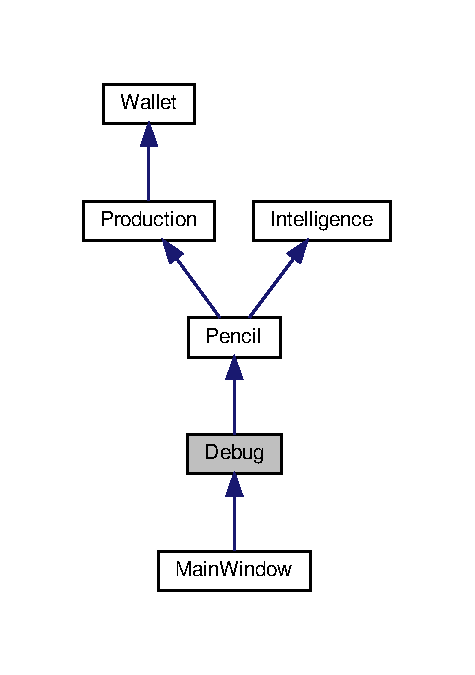
\includegraphics[width=228pt]{classDebug__inherit__graph}
\end{center}
\end{figure}


Collaboration diagram for Debug\+:\nopagebreak
\begin{figure}[H]
\begin{center}
\leavevmode
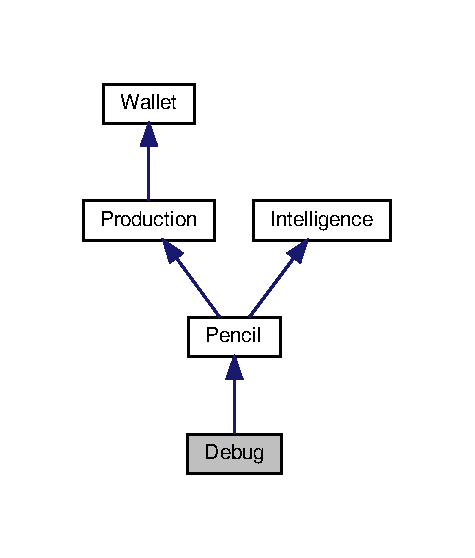
\includegraphics[width=228pt]{classDebug__coll__graph}
\end{center}
\end{figure}
\subsection*{Public Member Functions}
\begin{DoxyCompactItemize}
\item 
\hyperlink{classDebug_a5b453c195c4cfffed2702c3330f53a64}{Debug} ()
\item 
void \hyperlink{classDebug_a4c42705f755444daa2a22b000a561e01}{speed\+Up} ()
\end{DoxyCompactItemize}
\subsection*{Additional Inherited Members}


\subsection{Detailed Description}
Class to implement \hyperlink{classDebug}{Debug} functionality. 

We define the constructor, destructor and necessary methods. 

\subsection{Constructor \& Destructor Documentation}
\mbox{\Hypertarget{classDebug_a5b453c195c4cfffed2702c3330f53a64}\label{classDebug_a5b453c195c4cfffed2702c3330f53a64}} 
\index{Debug@{Debug}!Debug@{Debug}}
\index{Debug@{Debug}!Debug@{Debug}}
\subsubsection{\texorpdfstring{Debug()}{Debug()}}
{\footnotesize\ttfamily Debug\+::\+Debug (\begin{DoxyParamCaption}{ }\end{DoxyParamCaption})}

Constructor. 

\subsection{Member Function Documentation}
\mbox{\Hypertarget{classDebug_a4c42705f755444daa2a22b000a561e01}\label{classDebug_a4c42705f755444daa2a22b000a561e01}} 
\index{Debug@{Debug}!speed\+Up@{speed\+Up}}
\index{speed\+Up@{speed\+Up}!Debug@{Debug}}
\subsubsection{\texorpdfstring{speed\+Up()}{speedUp()}}
{\footnotesize\ttfamily void Debug\+::speed\+Up (\begin{DoxyParamCaption}{ }\end{DoxyParamCaption})}

Function to speed up the specified values. 

The documentation for this class was generated from the following files\+:\begin{DoxyCompactItemize}
\item 
/home/ezio/sprint3/se-\/03-\/team-\/06/se-\/04-\/team-\/16/src/\hyperlink{debug_8h}{debug.\+h}\item 
/home/ezio/sprint3/se-\/03-\/team-\/06/se-\/04-\/team-\/16/src/debug.\+cpp\end{DoxyCompactItemize}

\hypertarget{classIntelligence}{}\section{Intelligence Class Reference}
\label{classIntelligence}\index{Intelligence@{Intelligence}}


Class to implement \hyperlink{classIntelligence}{Intelligence} currency.  




{\ttfamily \#include $<$intelligence.\+h$>$}



Inheritance diagram for Intelligence\+:
% FIG 0
\subsection*{Public Member Functions}
\begin{DoxyCompactItemize}
\item 
\hyperlink{classIntelligence_a146fc36901bb5993c71b0d9426439fea}{Intelligence} ()
\item 
void \hyperlink{classIntelligence_ad822db7ef4eef6c1f797f65c73fec3f0}{increase\+Intelligence} ()
\end{DoxyCompactItemize}
\subsection*{Public Attributes}
\begin{DoxyCompactItemize}
\item 
int \hyperlink{classIntelligence_a20fc418262dd34db0d9e99d81d6a7544}{intelligence\+Balance}
\item 
\mbox{\Hypertarget{classIntelligence_ad8d4fda31beb86dc434f71fe6c683ae9}\label{classIntelligence_ad8d4fda31beb86dc434f71fe6c683ae9}} 
bool {\bfseries intelligence\+Is\+Active}
\end{DoxyCompactItemize}


\subsection{Detailed Description}
Class to implement \hyperlink{classIntelligence}{Intelligence} currency. 

We define the constructor and necessary methods. 

\subsection{Constructor \& Destructor Documentation}
\mbox{\Hypertarget{classIntelligence_a146fc36901bb5993c71b0d9426439fea}\label{classIntelligence_a146fc36901bb5993c71b0d9426439fea}} 
\index{Intelligence@{Intelligence}!Intelligence@{Intelligence}}
\index{Intelligence@{Intelligence}!Intelligence@{Intelligence}}
\subsubsection{\texorpdfstring{Intelligence()}{Intelligence()}}
{\footnotesize\ttfamily Intelligence\+::\+Intelligence (\begin{DoxyParamCaption}{ }\end{DoxyParamCaption})}

Constructor. 

\subsection{Member Function Documentation}
\mbox{\Hypertarget{classIntelligence_ad822db7ef4eef6c1f797f65c73fec3f0}\label{classIntelligence_ad822db7ef4eef6c1f797f65c73fec3f0}} 
\index{Intelligence@{Intelligence}!increase\+Intelligence@{increase\+Intelligence}}
\index{increase\+Intelligence@{increase\+Intelligence}!Intelligence@{Intelligence}}
\subsubsection{\texorpdfstring{increase\+Intelligence()}{increaseIntelligence()}}
{\footnotesize\ttfamily void Intelligence\+::increase\+Intelligence (\begin{DoxyParamCaption}{ }\end{DoxyParamCaption})}

Insert your comment here. 

\subsection{Member Data Documentation}
\mbox{\Hypertarget{classIntelligence_a20fc418262dd34db0d9e99d81d6a7544}\label{classIntelligence_a20fc418262dd34db0d9e99d81d6a7544}} 
\index{Intelligence@{Intelligence}!intelligence\+Balance@{intelligence\+Balance}}
\index{intelligence\+Balance@{intelligence\+Balance}!Intelligence@{Intelligence}}
\subsubsection{\texorpdfstring{intelligence\+Balance}{intelligenceBalance}}
{\footnotesize\ttfamily int Intelligence\+::intelligence\+Balance}

Insert your comment here. 

The documentation for this class was generated from the following files\+:\begin{DoxyCompactItemize}
\item 
/home/fatine/\+Documents/se-\/03-\/team-\/06/src/\hyperlink{intelligence_8h}{intelligence.\+h}\item 
/home/fatine/\+Documents/se-\/03-\/team-\/06/src/intelligence.\+cpp\end{DoxyCompactItemize}

\hypertarget{classMainWindow}{}\section{Main\+Window Class Reference}
\label{classMainWindow}\index{Main\+Window@{Main\+Window}}


Class to implement the \hyperlink{classMainWindow}{Main\+Window}.  




{\ttfamily \#include $<$mainwindow.\+h$>$}



Inheritance diagram for Main\+Window\+:
% FIG 0


Collaboration diagram for Main\+Window\+:
% FIG 1
\subsection*{Public Member Functions}
\begin{DoxyCompactItemize}
\item 
\hyperlink{classMainWindow_a996c5a2b6f77944776856f08ec30858d}{Main\+Window} (Q\+Widget $\ast$parent=nullptr)
\begin{DoxyCompactList}\small\item\em Mainwindow constructor. \end{DoxyCompactList}\item 
\hyperlink{classMainWindow_ae98d00a93bc118200eeef9f9bba1dba7}{$\sim$\+Main\+Window} ()
\end{DoxyCompactItemize}
\subsection*{Additional Inherited Members}


\subsection{Detailed Description}
Class to implement the \hyperlink{classMainWindow}{Main\+Window}. 

class \hyperlink{classMainWindow}{Main\+Window} extending from Q\+Main\+Window uses Q\+\_\+\+O\+B\+J\+E\+CT macro defined in Q\+Main\+Window header 

\subsection{Constructor \& Destructor Documentation}
\mbox{\Hypertarget{classMainWindow_a996c5a2b6f77944776856f08ec30858d}\label{classMainWindow_a996c5a2b6f77944776856f08ec30858d}} 
\index{Main\+Window@{Main\+Window}!Main\+Window@{Main\+Window}}
\index{Main\+Window@{Main\+Window}!Main\+Window@{Main\+Window}}
\subsubsection{\texorpdfstring{Main\+Window()}{MainWindow()}}
{\footnotesize\ttfamily Main\+Window\+::\+Main\+Window (\begin{DoxyParamCaption}\item[{Q\+Widget $\ast$}]{parent = {\ttfamily nullptr} }\end{DoxyParamCaption})\hspace{0.3cm}{\ttfamily [explicit]}}



Mainwindow constructor. 

Constructor. Label is set to display as soon as the \hyperlink{classMainWindow}{Main\+Window} class is constructed.

Timer initialization.

This timer is used for calculating prices of graphite and wood every 5 sec.

Action to be taken when save is clicked

Action to be taken when load is clicked

Not displaying the debugging tool option

Not displaying the debugging tool

Action to be taken when debug is clicked

Action to be taken when speed up is clicked\mbox{\Hypertarget{classMainWindow_ae98d00a93bc118200eeef9f9bba1dba7}\label{classMainWindow_ae98d00a93bc118200eeef9f9bba1dba7}} 
\index{Main\+Window@{Main\+Window}!````~Main\+Window@{$\sim$\+Main\+Window}}
\index{````~Main\+Window@{$\sim$\+Main\+Window}!Main\+Window@{Main\+Window}}
\subsubsection{\texorpdfstring{$\sim$\+Main\+Window()}{~MainWindow()}}
{\footnotesize\ttfamily Main\+Window\+::$\sim$\+Main\+Window (\begin{DoxyParamCaption}{ }\end{DoxyParamCaption})}

Destructor. 

The documentation for this class was generated from the following files\+:\begin{DoxyCompactItemize}
\item 
/home/fatine/\+Documents/se-\/03-\/team-\/06/src/\hyperlink{mainwindow_8h}{mainwindow.\+h}\item 
/home/fatine/\+Documents/se-\/03-\/team-\/06/src/mainwindow.\+cpp\end{DoxyCompactItemize}

\hypertarget{classPencil}{}\section{Pencil Class Reference}
\label{classPencil}\index{Pencil@{Pencil}}


Class to implement pencil game.  




{\ttfamily \#include $<$pencil.\+h$>$}



Inheritance diagram for Pencil\+:
\nopagebreak
\begin{figure}[H]
\begin{center}
\leavevmode
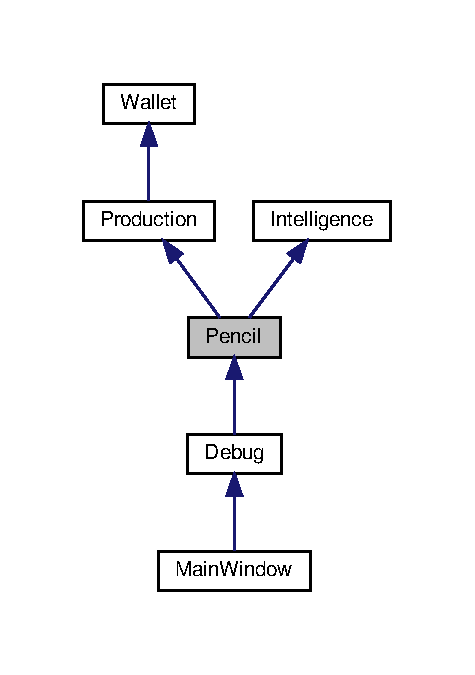
\includegraphics[width=228pt]{classPencil__inherit__graph}
\end{center}
\end{figure}


Collaboration diagram for Pencil\+:
\nopagebreak
\begin{figure}[H]
\begin{center}
\leavevmode
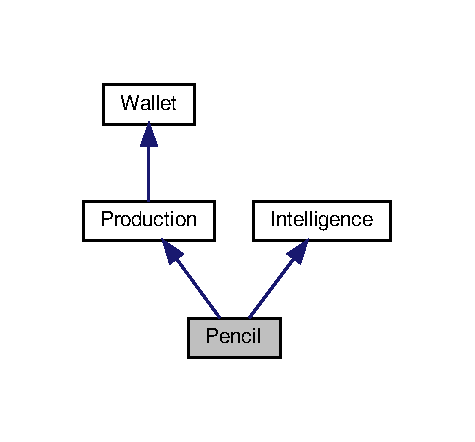
\includegraphics[width=228pt]{classPencil__coll__graph}
\end{center}
\end{figure}
\subsection*{Public Member Functions}
\begin{DoxyCompactItemize}
\item 
\hyperlink{classPencil_a0dbfad3eebde26e9d5dacace449d9e14}{Pencil} ()
\item 
void \hyperlink{classPencil_a582594d67f32d7cb427f1bbe2824382b}{initialize\+Pencil} ()
\item 
int \hyperlink{classPencil_aa629f185016565c847bb0a401634f0e5}{get\+Inventory} ()
\item 
void \hyperlink{classPencil_ae966b635fd81f8d346aaa7f8f782f143}{produce\+Pencil} ()
\item 
void \hyperlink{classPencil_a075683b2e85f8819e71f365c097e5f61}{increase\+Price} ()
\item 
void \hyperlink{classPencil_a84aeeb98b1caa424d92c312e56e42797}{decrease\+Price} ()
\item 
void \hyperlink{classPencil_a2731dadbd64edeee0a1cc773a79eee24}{sell} ()
\item 
void \hyperlink{classPencil_a759af90fe58f6399e831f2c53c0470bd}{new\+Rate} ()
\item 
void \hyperlink{classPencil_a506c7c9587a026f1238e880b1b103c2f}{buy\+Apm} ()
\item 
void \hyperlink{classPencil_ad1f8942401865e05d2a220f64a309f3e}{apm2000} ()
\item 
void \hyperlink{classPencil_aaeb664bbf0ab3796bc548eccee5924ed}{upgrade\+Apm} ()
\item 
double \hyperlink{classPencil_a9bbb66405447f4cc218ecbd1a09b7c3b}{round} (double var)
\item 
void \hyperlink{classPencil_a4d1fff5599020013b3b52cf84d714847}{upgrade\+Marketing} ()
\end{DoxyCompactItemize}
\subsection*{Public Attributes}
\begin{DoxyCompactItemize}
\item 
double \hyperlink{classPencil_a71779a08ea791bf285d7e7d901d49d96}{priceof\+Pencil}
\item 
double \hyperlink{classPencil_acc8e87622507eb7d7b6802c561bbf4b5}{rateof\+Pencil}
\item 
int \hyperlink{classPencil_a42f809cbd4230815aed7212fe148367c}{numberof\+Pencil}
\item 
double \hyperlink{classPencil_a80b094bc36884ba078bc6e07c56871af}{totalnumberof\+Pencil}
\item 
int \hyperlink{classPencil_a0af93e74decc39b154f1248c2a987809}{pencils\+For\+Upgrade}
\item 
double \hyperlink{classPencil_a07127489c562b29b05f439ea380db9d0}{numberof\+Apm}
\item 
double \hyperlink{classPencil_a34a1a763466d2ea7408bf470adcf63f2}{priceof\+Apm}
\item 
double \hyperlink{classPencil_a5b8822d01032897b432fff6ac20d6fb5}{rateof\+Apm}
\item 
double \hyperlink{classPencil_a71b50db432298677e50884b34002bbcf}{apm\+Fractional}
\item 
int \hyperlink{classPencil_a1f05477be34cb47d39c3888fb1c4092c}{apm\+Upgrade\+Price}
\item 
bool \hyperlink{classPencil_a3d54aa5bf47e0f850640098fe1f64730}{apm\+Upgrade\+Available}
\item 
int \hyperlink{classPencil_a1bc69bd5b4a595710c48d68a2d276044}{marketing}
\item 
double \hyperlink{classPencil_a4d8be35743fd0687fcc95a4643594568}{marketing\+Upgrade\+Price}
\item 
bool \hyperlink{classPencil_a180f62c45b0d40ea3ef84038e40d1f55}{marketing\+Unlocked}
\end{DoxyCompactItemize}


\subsection{Detailed Description}
Class to implement pencil game. 

We define the constructor, variables and necessary methods. 

\subsection{Constructor \& Destructor Documentation}
\mbox{\Hypertarget{classPencil_a0dbfad3eebde26e9d5dacace449d9e14}\label{classPencil_a0dbfad3eebde26e9d5dacace449d9e14}} 
\index{Pencil@{Pencil}!Pencil@{Pencil}}
\index{Pencil@{Pencil}!Pencil@{Pencil}}
\subsubsection{\texorpdfstring{Pencil()}{Pencil()}}
{\footnotesize\ttfamily Pencil\+::\+Pencil (\begin{DoxyParamCaption}{ }\end{DoxyParamCaption})}

Constructor. 

\subsection{Member Function Documentation}
\mbox{\Hypertarget{classPencil_ad1f8942401865e05d2a220f64a309f3e}\label{classPencil_ad1f8942401865e05d2a220f64a309f3e}} 
\index{Pencil@{Pencil}!apm2000@{apm2000}}
\index{apm2000@{apm2000}!Pencil@{Pencil}}
\subsubsection{\texorpdfstring{apm2000()}{apm2000()}}
{\footnotesize\ttfamily void Pencil\+::apm2000 (\begin{DoxyParamCaption}{ }\end{DoxyParamCaption})}

A\+PM 2000.

Function to produce pencils for the A\+PM \mbox{\Hypertarget{classPencil_a506c7c9587a026f1238e880b1b103c2f}\label{classPencil_a506c7c9587a026f1238e880b1b103c2f}} 
\index{Pencil@{Pencil}!buy\+Apm@{buy\+Apm}}
\index{buy\+Apm@{buy\+Apm}!Pencil@{Pencil}}
\subsubsection{\texorpdfstring{buy\+Apm()}{buyApm()}}
{\footnotesize\ttfamily void Pencil\+::buy\+Apm (\begin{DoxyParamCaption}{ }\end{DoxyParamCaption})}

Buy A\+PM.

Function to buy A\+PM and increase its price by 10\% after every purchase \mbox{\Hypertarget{classPencil_a84aeeb98b1caa424d92c312e56e42797}\label{classPencil_a84aeeb98b1caa424d92c312e56e42797}} 
\index{Pencil@{Pencil}!decrease\+Price@{decrease\+Price}}
\index{decrease\+Price@{decrease\+Price}!Pencil@{Pencil}}
\subsubsection{\texorpdfstring{decrease\+Price()}{decreasePrice()}}
{\footnotesize\ttfamily void Pencil\+::decrease\+Price (\begin{DoxyParamCaption}{ }\end{DoxyParamCaption})}

Decrease price of pencil. \mbox{\Hypertarget{classPencil_aa629f185016565c847bb0a401634f0e5}\label{classPencil_aa629f185016565c847bb0a401634f0e5}} 
\index{Pencil@{Pencil}!get\+Inventory@{get\+Inventory}}
\index{get\+Inventory@{get\+Inventory}!Pencil@{Pencil}}
\subsubsection{\texorpdfstring{get\+Inventory()}{getInventory()}}
{\footnotesize\ttfamily int Pencil\+::get\+Inventory (\begin{DoxyParamCaption}{ }\end{DoxyParamCaption})}

Returns pencils in invertory. \mbox{\Hypertarget{classPencil_a075683b2e85f8819e71f365c097e5f61}\label{classPencil_a075683b2e85f8819e71f365c097e5f61}} 
\index{Pencil@{Pencil}!increase\+Price@{increase\+Price}}
\index{increase\+Price@{increase\+Price}!Pencil@{Pencil}}
\subsubsection{\texorpdfstring{increase\+Price()}{increasePrice()}}
{\footnotesize\ttfamily void Pencil\+::increase\+Price (\begin{DoxyParamCaption}{ }\end{DoxyParamCaption})}

Increase price of pencil. \mbox{\Hypertarget{classPencil_a582594d67f32d7cb427f1bbe2824382b}\label{classPencil_a582594d67f32d7cb427f1bbe2824382b}} 
\index{Pencil@{Pencil}!initialize\+Pencil@{initialize\+Pencil}}
\index{initialize\+Pencil@{initialize\+Pencil}!Pencil@{Pencil}}
\subsubsection{\texorpdfstring{initialize\+Pencil()}{initializePencil()}}
{\footnotesize\ttfamily void Pencil\+::initialize\+Pencil (\begin{DoxyParamCaption}{ }\end{DoxyParamCaption})}

Initializes class variables \mbox{\Hypertarget{classPencil_a759af90fe58f6399e831f2c53c0470bd}\label{classPencil_a759af90fe58f6399e831f2c53c0470bd}} 
\index{Pencil@{Pencil}!new\+Rate@{new\+Rate}}
\index{new\+Rate@{new\+Rate}!Pencil@{Pencil}}
\subsubsection{\texorpdfstring{new\+Rate()}{newRate()}}
{\footnotesize\ttfamily void Pencil\+::new\+Rate (\begin{DoxyParamCaption}{ }\end{DoxyParamCaption})}

New rate of pencil sells.

Function to calculate rate of a pencil every 0.\+20 seconds \mbox{\Hypertarget{classPencil_ae966b635fd81f8d346aaa7f8f782f143}\label{classPencil_ae966b635fd81f8d346aaa7f8f782f143}} 
\index{Pencil@{Pencil}!produce\+Pencil@{produce\+Pencil}}
\index{produce\+Pencil@{produce\+Pencil}!Pencil@{Pencil}}
\subsubsection{\texorpdfstring{produce\+Pencil()}{producePencil()}}
{\footnotesize\ttfamily void Pencil\+::produce\+Pencil (\begin{DoxyParamCaption}{ }\end{DoxyParamCaption})}

Produce pencils. \mbox{\Hypertarget{classPencil_a9bbb66405447f4cc218ecbd1a09b7c3b}\label{classPencil_a9bbb66405447f4cc218ecbd1a09b7c3b}} 
\index{Pencil@{Pencil}!round@{round}}
\index{round@{round}!Pencil@{Pencil}}
\subsubsection{\texorpdfstring{round()}{round()}}
{\footnotesize\ttfamily double Pencil\+::round (\begin{DoxyParamCaption}\item[{double}]{var }\end{DoxyParamCaption})}

Function to round number to 2 decimal places.

Function to round doubles to two decimal places \mbox{\Hypertarget{classPencil_a2731dadbd64edeee0a1cc773a79eee24}\label{classPencil_a2731dadbd64edeee0a1cc773a79eee24}} 
\index{Pencil@{Pencil}!sell@{sell}}
\index{sell@{sell}!Pencil@{Pencil}}
\subsubsection{\texorpdfstring{sell()}{sell()}}
{\footnotesize\ttfamily void Pencil\+::sell (\begin{DoxyParamCaption}{ }\end{DoxyParamCaption})}

Sells pencil.

Sell pencils (according to rate) every second Selling pencils in bulk \mbox{\Hypertarget{classPencil_aaeb664bbf0ab3796bc548eccee5924ed}\label{classPencil_aaeb664bbf0ab3796bc548eccee5924ed}} 
\index{Pencil@{Pencil}!upgrade\+Apm@{upgrade\+Apm}}
\index{upgrade\+Apm@{upgrade\+Apm}!Pencil@{Pencil}}
\subsubsection{\texorpdfstring{upgrade\+Apm()}{upgradeApm()}}
{\footnotesize\ttfamily void Pencil\+::upgrade\+Apm (\begin{DoxyParamCaption}{ }\end{DoxyParamCaption})}

Upgrade of A\+PM.

Function to upgrade A\+PM \mbox{\Hypertarget{classPencil_a4d1fff5599020013b3b52cf84d714847}\label{classPencil_a4d1fff5599020013b3b52cf84d714847}} 
\index{Pencil@{Pencil}!upgrade\+Marketing@{upgrade\+Marketing}}
\index{upgrade\+Marketing@{upgrade\+Marketing}!Pencil@{Pencil}}
\subsubsection{\texorpdfstring{upgrade\+Marketing()}{upgradeMarketing()}}
{\footnotesize\ttfamily void Pencil\+::upgrade\+Marketing (\begin{DoxyParamCaption}{ }\end{DoxyParamCaption})}

Function to upgrade market.

Function to upgrade marketing and adjust upgrade price 

\subsection{Member Data Documentation}
\mbox{\Hypertarget{classPencil_a71b50db432298677e50884b34002bbcf}\label{classPencil_a71b50db432298677e50884b34002bbcf}} 
\index{Pencil@{Pencil}!apm\+Fractional@{apm\+Fractional}}
\index{apm\+Fractional@{apm\+Fractional}!Pencil@{Pencil}}
\subsubsection{\texorpdfstring{apm\+Fractional}{apmFractional}}
{\footnotesize\ttfamily double Pencil\+::apm\+Fractional}

A\+PM fractional. \mbox{\Hypertarget{classPencil_a3d54aa5bf47e0f850640098fe1f64730}\label{classPencil_a3d54aa5bf47e0f850640098fe1f64730}} 
\index{Pencil@{Pencil}!apm\+Upgrade\+Available@{apm\+Upgrade\+Available}}
\index{apm\+Upgrade\+Available@{apm\+Upgrade\+Available}!Pencil@{Pencil}}
\subsubsection{\texorpdfstring{apm\+Upgrade\+Available}{apmUpgradeAvailable}}
{\footnotesize\ttfamily bool Pencil\+::apm\+Upgrade\+Available}

A\+PM upgrade availability. \mbox{\Hypertarget{classPencil_a1f05477be34cb47d39c3888fb1c4092c}\label{classPencil_a1f05477be34cb47d39c3888fb1c4092c}} 
\index{Pencil@{Pencil}!apm\+Upgrade\+Price@{apm\+Upgrade\+Price}}
\index{apm\+Upgrade\+Price@{apm\+Upgrade\+Price}!Pencil@{Pencil}}
\subsubsection{\texorpdfstring{apm\+Upgrade\+Price}{apmUpgradePrice}}
{\footnotesize\ttfamily int Pencil\+::apm\+Upgrade\+Price}

Price of A\+PM. \mbox{\Hypertarget{classPencil_a1bc69bd5b4a595710c48d68a2d276044}\label{classPencil_a1bc69bd5b4a595710c48d68a2d276044}} 
\index{Pencil@{Pencil}!marketing@{marketing}}
\index{marketing@{marketing}!Pencil@{Pencil}}
\subsubsection{\texorpdfstring{marketing}{marketing}}
{\footnotesize\ttfamily int Pencil\+::marketing}

Marketing price. \mbox{\Hypertarget{classPencil_a180f62c45b0d40ea3ef84038e40d1f55}\label{classPencil_a180f62c45b0d40ea3ef84038e40d1f55}} 
\index{Pencil@{Pencil}!marketing\+Unlocked@{marketing\+Unlocked}}
\index{marketing\+Unlocked@{marketing\+Unlocked}!Pencil@{Pencil}}
\subsubsection{\texorpdfstring{marketing\+Unlocked}{marketingUnlocked}}
{\footnotesize\ttfamily bool Pencil\+::marketing\+Unlocked}

Marketing functionality (active/inactive) \mbox{\Hypertarget{classPencil_a4d8be35743fd0687fcc95a4643594568}\label{classPencil_a4d8be35743fd0687fcc95a4643594568}} 
\index{Pencil@{Pencil}!marketing\+Upgrade\+Price@{marketing\+Upgrade\+Price}}
\index{marketing\+Upgrade\+Price@{marketing\+Upgrade\+Price}!Pencil@{Pencil}}
\subsubsection{\texorpdfstring{marketing\+Upgrade\+Price}{marketingUpgradePrice}}
{\footnotesize\ttfamily double Pencil\+::marketing\+Upgrade\+Price}

Marketing price upgrade. \mbox{\Hypertarget{classPencil_a07127489c562b29b05f439ea380db9d0}\label{classPencil_a07127489c562b29b05f439ea380db9d0}} 
\index{Pencil@{Pencil}!numberof\+Apm@{numberof\+Apm}}
\index{numberof\+Apm@{numberof\+Apm}!Pencil@{Pencil}}
\subsubsection{\texorpdfstring{numberof\+Apm}{numberofApm}}
{\footnotesize\ttfamily double Pencil\+::numberof\+Apm}

Number of A\+P\+Ms. \mbox{\Hypertarget{classPencil_a42f809cbd4230815aed7212fe148367c}\label{classPencil_a42f809cbd4230815aed7212fe148367c}} 
\index{Pencil@{Pencil}!numberof\+Pencil@{numberof\+Pencil}}
\index{numberof\+Pencil@{numberof\+Pencil}!Pencil@{Pencil}}
\subsubsection{\texorpdfstring{numberof\+Pencil}{numberofPencil}}
{\footnotesize\ttfamily int Pencil\+::numberof\+Pencil}

Number of pencil produced. \mbox{\Hypertarget{classPencil_a0af93e74decc39b154f1248c2a987809}\label{classPencil_a0af93e74decc39b154f1248c2a987809}} 
\index{Pencil@{Pencil}!pencils\+For\+Upgrade@{pencils\+For\+Upgrade}}
\index{pencils\+For\+Upgrade@{pencils\+For\+Upgrade}!Pencil@{Pencil}}
\subsubsection{\texorpdfstring{pencils\+For\+Upgrade}{pencilsForUpgrade}}
{\footnotesize\ttfamily int Pencil\+::pencils\+For\+Upgrade}

Pencils for upgrade. \mbox{\Hypertarget{classPencil_a34a1a763466d2ea7408bf470adcf63f2}\label{classPencil_a34a1a763466d2ea7408bf470adcf63f2}} 
\index{Pencil@{Pencil}!priceof\+Apm@{priceof\+Apm}}
\index{priceof\+Apm@{priceof\+Apm}!Pencil@{Pencil}}
\subsubsection{\texorpdfstring{priceof\+Apm}{priceofApm}}
{\footnotesize\ttfamily double Pencil\+::priceof\+Apm}

Price of A\+P\+Ms. \mbox{\Hypertarget{classPencil_a71779a08ea791bf285d7e7d901d49d96}\label{classPencil_a71779a08ea791bf285d7e7d901d49d96}} 
\index{Pencil@{Pencil}!priceof\+Pencil@{priceof\+Pencil}}
\index{priceof\+Pencil@{priceof\+Pencil}!Pencil@{Pencil}}
\subsubsection{\texorpdfstring{priceof\+Pencil}{priceofPencil}}
{\footnotesize\ttfamily double Pencil\+::priceof\+Pencil}

Price of pencil. \mbox{\Hypertarget{classPencil_a5b8822d01032897b432fff6ac20d6fb5}\label{classPencil_a5b8822d01032897b432fff6ac20d6fb5}} 
\index{Pencil@{Pencil}!rateof\+Apm@{rateof\+Apm}}
\index{rateof\+Apm@{rateof\+Apm}!Pencil@{Pencil}}
\subsubsection{\texorpdfstring{rateof\+Apm}{rateofApm}}
{\footnotesize\ttfamily double Pencil\+::rateof\+Apm}

Rate of A\+P\+Ms. \mbox{\Hypertarget{classPencil_acc8e87622507eb7d7b6802c561bbf4b5}\label{classPencil_acc8e87622507eb7d7b6802c561bbf4b5}} 
\index{Pencil@{Pencil}!rateof\+Pencil@{rateof\+Pencil}}
\index{rateof\+Pencil@{rateof\+Pencil}!Pencil@{Pencil}}
\subsubsection{\texorpdfstring{rateof\+Pencil}{rateofPencil}}
{\footnotesize\ttfamily double Pencil\+::rateof\+Pencil}

Sell rate of pencil. \mbox{\Hypertarget{classPencil_a80b094bc36884ba078bc6e07c56871af}\label{classPencil_a80b094bc36884ba078bc6e07c56871af}} 
\index{Pencil@{Pencil}!totalnumberof\+Pencil@{totalnumberof\+Pencil}}
\index{totalnumberof\+Pencil@{totalnumberof\+Pencil}!Pencil@{Pencil}}
\subsubsection{\texorpdfstring{totalnumberof\+Pencil}{totalnumberofPencil}}
{\footnotesize\ttfamily double Pencil\+::totalnumberof\+Pencil}

Total number of pencil produced. 

The documentation for this class was generated from the following files\+:\begin{DoxyCompactItemize}
\item 
/home/ezio/sprint3/se-\/03-\/team-\/06/se-\/04-\/team-\/16/src/\hyperlink{pencil_8h}{pencil.\+h}\item 
/home/ezio/sprint3/se-\/03-\/team-\/06/se-\/04-\/team-\/16/src/pencil.\+cpp\end{DoxyCompactItemize}

\hypertarget{classProduction}{}\section{Production Class Reference}
\label{classProduction}\index{Production@{Production}}


Class to implement production of the pencils.  




{\ttfamily \#include $<$production.\+h$>$}



Inheritance diagram for Production\+:
\nopagebreak
\begin{figure}[H]
\begin{center}
\leavevmode
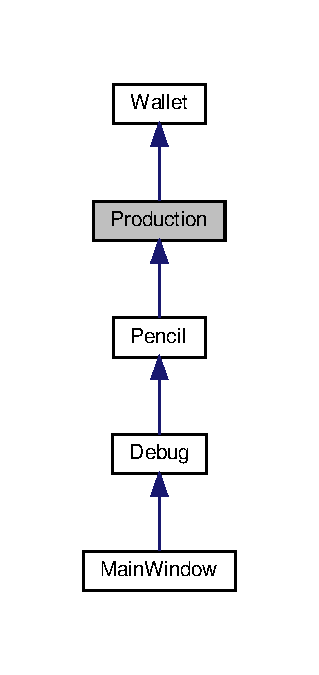
\includegraphics[width=153pt]{classProduction__inherit__graph}
\end{center}
\end{figure}


Collaboration diagram for Production\+:
\nopagebreak
\begin{figure}[H]
\begin{center}
\leavevmode
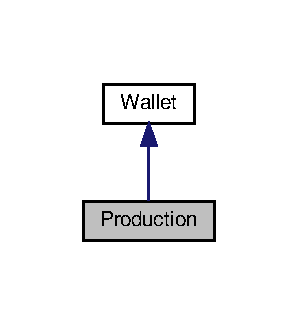
\includegraphics[width=143pt]{classProduction__coll__graph}
\end{center}
\end{figure}
\subsection*{Public Member Functions}
\begin{DoxyCompactItemize}
\item 
\hyperlink{classProduction_a12c7c685be71ed51ac10f7d0284e8d4f}{Production} ()
\item 
void \hyperlink{classProduction_ae3559bf477b74d73fa6332b59f70ed2a}{initialize\+Production} ()
\item 
void \hyperlink{classProduction_a5eea7af1f4949832bcc0c019f420d655}{buy\+Wood} ()
\item 
void \hyperlink{classProduction_adf62fb3241254aa3412ed9a9d1fb27a2}{buy\+Graphite} ()
\item 
bool \hyperlink{classProduction_a5f5c38b7f3f7b23f9029d562c7e53025}{disable\+\_\+buy\+Wood} ()
\item 
bool \hyperlink{classProduction_a4c87c63f0fdc741f9185dcda6793463e}{disable\+\_\+buy\+Graphite} ()
\item 
void \hyperlink{classProduction_a4a9bbd94b71b1d24d836d9ad79bed97b}{calculate\+Prices} ()
\item 
void \hyperlink{classProduction_a42c46b93e65cb3f84db76562a27d44f6}{decrease\+Wood} ()
\item 
void \hyperlink{classProduction_aa5180ed4aac0e3d8ecec30596c9b1751}{decrease\+Graphite} ()
\item 
double \hyperlink{classProduction_a8991aa503f8d94ae01ff9b7f08043c58}{get\+Wood} ()
\item 
double \hyperlink{classProduction_ad8e6b675848c58fcf04e214e383a87fd}{get\+Graphite} ()
\end{DoxyCompactItemize}
\subsection*{Public Attributes}
\begin{DoxyCompactItemize}
\item 
double \hyperlink{classProduction_ac6bc16863f128802bebbb52263d5558c}{priceof\+Wood}
\item 
double \hyperlink{classProduction_afca6aca1df88921b60bb7190adab5d51}{priceof\+Graphite}
\item 
double \hyperlink{classProduction_a5d77a106ee08bfb55522cdd28e0d364e}{numberof\+Wood}
\item 
double \hyperlink{classProduction_a3b0d11cefec32eeec83637e1d5252a41}{numberof\+Graphite}
\end{DoxyCompactItemize}


\subsection{Detailed Description}
Class to implement production of the pencils. 

We define the constructor, variables and necessary methods. 

\subsection{Constructor \& Destructor Documentation}
\mbox{\Hypertarget{classProduction_a12c7c685be71ed51ac10f7d0284e8d4f}\label{classProduction_a12c7c685be71ed51ac10f7d0284e8d4f}} 
\index{Production@{Production}!Production@{Production}}
\index{Production@{Production}!Production@{Production}}
\subsubsection{\texorpdfstring{Production()}{Production()}}
{\footnotesize\ttfamily Production\+::\+Production (\begin{DoxyParamCaption}{ }\end{DoxyParamCaption})}

Constructor. 

\subsection{Member Function Documentation}
\mbox{\Hypertarget{classProduction_adf62fb3241254aa3412ed9a9d1fb27a2}\label{classProduction_adf62fb3241254aa3412ed9a9d1fb27a2}} 
\index{Production@{Production}!buy\+Graphite@{buy\+Graphite}}
\index{buy\+Graphite@{buy\+Graphite}!Production@{Production}}
\subsubsection{\texorpdfstring{buy\+Graphite()}{buyGraphite()}}
{\footnotesize\ttfamily void Production\+::buy\+Graphite (\begin{DoxyParamCaption}{ }\end{DoxyParamCaption})}

Buy graphite function.

Function to buy Graphite if there is enough balance \mbox{\Hypertarget{classProduction_a5eea7af1f4949832bcc0c019f420d655}\label{classProduction_a5eea7af1f4949832bcc0c019f420d655}} 
\index{Production@{Production}!buy\+Wood@{buy\+Wood}}
\index{buy\+Wood@{buy\+Wood}!Production@{Production}}
\subsubsection{\texorpdfstring{buy\+Wood()}{buyWood()}}
{\footnotesize\ttfamily void Production\+::buy\+Wood (\begin{DoxyParamCaption}{ }\end{DoxyParamCaption})}

Buy wood function.

Function to buy wood if there is enough balance \mbox{\Hypertarget{classProduction_a4a9bbd94b71b1d24d836d9ad79bed97b}\label{classProduction_a4a9bbd94b71b1d24d836d9ad79bed97b}} 
\index{Production@{Production}!calculate\+Prices@{calculate\+Prices}}
\index{calculate\+Prices@{calculate\+Prices}!Production@{Production}}
\subsubsection{\texorpdfstring{calculate\+Prices()}{calculatePrices()}}
{\footnotesize\ttfamily void Production\+::calculate\+Prices (\begin{DoxyParamCaption}{ }\end{DoxyParamCaption})}

Calculates price of wood and graphite function.

Function to calculate price of Wood and Graphite. Price of Wood and Graphite is a random number between 1000 to 2000.

Price of Graphite is a random number between 1500 to 2500. \mbox{\Hypertarget{classProduction_aa5180ed4aac0e3d8ecec30596c9b1751}\label{classProduction_aa5180ed4aac0e3d8ecec30596c9b1751}} 
\index{Production@{Production}!decrease\+Graphite@{decrease\+Graphite}}
\index{decrease\+Graphite@{decrease\+Graphite}!Production@{Production}}
\subsubsection{\texorpdfstring{decrease\+Graphite()}{decreaseGraphite()}}
{\footnotesize\ttfamily void Production\+::decrease\+Graphite (\begin{DoxyParamCaption}{ }\end{DoxyParamCaption})}

Consume graphite function. \mbox{\Hypertarget{classProduction_a42c46b93e65cb3f84db76562a27d44f6}\label{classProduction_a42c46b93e65cb3f84db76562a27d44f6}} 
\index{Production@{Production}!decrease\+Wood@{decrease\+Wood}}
\index{decrease\+Wood@{decrease\+Wood}!Production@{Production}}
\subsubsection{\texorpdfstring{decrease\+Wood()}{decreaseWood()}}
{\footnotesize\ttfamily void Production\+::decrease\+Wood (\begin{DoxyParamCaption}{ }\end{DoxyParamCaption})}

Consumes wood function. \mbox{\Hypertarget{classProduction_a4c87c63f0fdc741f9185dcda6793463e}\label{classProduction_a4c87c63f0fdc741f9185dcda6793463e}} 
\index{Production@{Production}!disable\+\_\+buy\+Graphite@{disable\+\_\+buy\+Graphite}}
\index{disable\+\_\+buy\+Graphite@{disable\+\_\+buy\+Graphite}!Production@{Production}}
\subsubsection{\texorpdfstring{disable\+\_\+buy\+Graphite()}{disable\_buyGraphite()}}
{\footnotesize\ttfamily bool Production\+::disable\+\_\+buy\+Graphite (\begin{DoxyParamCaption}{ }\end{DoxyParamCaption})}

Disable buy graphite function. \mbox{\Hypertarget{classProduction_a5f5c38b7f3f7b23f9029d562c7e53025}\label{classProduction_a5f5c38b7f3f7b23f9029d562c7e53025}} 
\index{Production@{Production}!disable\+\_\+buy\+Wood@{disable\+\_\+buy\+Wood}}
\index{disable\+\_\+buy\+Wood@{disable\+\_\+buy\+Wood}!Production@{Production}}
\subsubsection{\texorpdfstring{disable\+\_\+buy\+Wood()}{disable\_buyWood()}}
{\footnotesize\ttfamily bool Production\+::disable\+\_\+buy\+Wood (\begin{DoxyParamCaption}{ }\end{DoxyParamCaption})}

Disable buy wood function. \mbox{\Hypertarget{classProduction_ad8e6b675848c58fcf04e214e383a87fd}\label{classProduction_ad8e6b675848c58fcf04e214e383a87fd}} 
\index{Production@{Production}!get\+Graphite@{get\+Graphite}}
\index{get\+Graphite@{get\+Graphite}!Production@{Production}}
\subsubsection{\texorpdfstring{get\+Graphite()}{getGraphite()}}
{\footnotesize\ttfamily double Production\+::get\+Graphite (\begin{DoxyParamCaption}{ }\end{DoxyParamCaption})}

return number of graphite. \mbox{\Hypertarget{classProduction_a8991aa503f8d94ae01ff9b7f08043c58}\label{classProduction_a8991aa503f8d94ae01ff9b7f08043c58}} 
\index{Production@{Production}!get\+Wood@{get\+Wood}}
\index{get\+Wood@{get\+Wood}!Production@{Production}}
\subsubsection{\texorpdfstring{get\+Wood()}{getWood()}}
{\footnotesize\ttfamily double Production\+::get\+Wood (\begin{DoxyParamCaption}{ }\end{DoxyParamCaption})}

return number of wood. \mbox{\Hypertarget{classProduction_ae3559bf477b74d73fa6332b59f70ed2a}\label{classProduction_ae3559bf477b74d73fa6332b59f70ed2a}} 
\index{Production@{Production}!initialize\+Production@{initialize\+Production}}
\index{initialize\+Production@{initialize\+Production}!Production@{Production}}
\subsubsection{\texorpdfstring{initialize\+Production()}{initializeProduction()}}
{\footnotesize\ttfamily void Production\+::initialize\+Production (\begin{DoxyParamCaption}{ }\end{DoxyParamCaption})}

Initializes class variables 

\subsection{Member Data Documentation}
\mbox{\Hypertarget{classProduction_a3b0d11cefec32eeec83637e1d5252a41}\label{classProduction_a3b0d11cefec32eeec83637e1d5252a41}} 
\index{Production@{Production}!numberof\+Graphite@{numberof\+Graphite}}
\index{numberof\+Graphite@{numberof\+Graphite}!Production@{Production}}
\subsubsection{\texorpdfstring{numberof\+Graphite}{numberofGraphite}}
{\footnotesize\ttfamily double Production\+::numberof\+Graphite}

Amount of graphite. \mbox{\Hypertarget{classProduction_a5d77a106ee08bfb55522cdd28e0d364e}\label{classProduction_a5d77a106ee08bfb55522cdd28e0d364e}} 
\index{Production@{Production}!numberof\+Wood@{numberof\+Wood}}
\index{numberof\+Wood@{numberof\+Wood}!Production@{Production}}
\subsubsection{\texorpdfstring{numberof\+Wood}{numberofWood}}
{\footnotesize\ttfamily double Production\+::numberof\+Wood}

Amount of wood. \mbox{\Hypertarget{classProduction_afca6aca1df88921b60bb7190adab5d51}\label{classProduction_afca6aca1df88921b60bb7190adab5d51}} 
\index{Production@{Production}!priceof\+Graphite@{priceof\+Graphite}}
\index{priceof\+Graphite@{priceof\+Graphite}!Production@{Production}}
\subsubsection{\texorpdfstring{priceof\+Graphite}{priceofGraphite}}
{\footnotesize\ttfamily double Production\+::priceof\+Graphite}

Price of Graphite. \mbox{\Hypertarget{classProduction_ac6bc16863f128802bebbb52263d5558c}\label{classProduction_ac6bc16863f128802bebbb52263d5558c}} 
\index{Production@{Production}!priceof\+Wood@{priceof\+Wood}}
\index{priceof\+Wood@{priceof\+Wood}!Production@{Production}}
\subsubsection{\texorpdfstring{priceof\+Wood}{priceofWood}}
{\footnotesize\ttfamily double Production\+::priceof\+Wood}

Price of Wood. 

The documentation for this class was generated from the following files\+:\begin{DoxyCompactItemize}
\item 
/home/ezio/sprint3/se-\/03-\/team-\/06/se-\/04-\/team-\/16/src/\hyperlink{production_8h}{production.\+h}\item 
/home/ezio/sprint3/se-\/03-\/team-\/06/se-\/04-\/team-\/16/src/production.\+cpp\end{DoxyCompactItemize}

\hypertarget{classServer}{}\section{Server Class Reference}
\label{classServer}\index{Server@{Server}}


Class to upload scores to server and acquire highscores from server.  




{\ttfamily \#include $<$server.\+h$>$}



Inheritance diagram for Server\+:\nopagebreak
\begin{figure}[H]
\begin{center}
\leavevmode
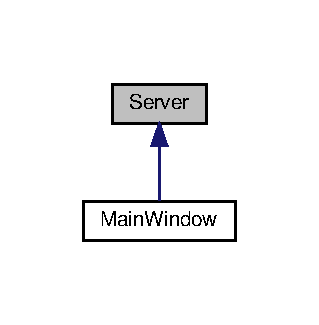
\includegraphics[width=153pt]{classServer__inherit__graph}
\end{center}
\end{figure}
\subsection*{Public Member Functions}
\begin{DoxyCompactItemize}
\item 
bool \hyperlink{classServer_a1675e8a33c0e4f9f2d51d3de16981e66}{upload\+Score} (int totalnumberof\+Pencil)
\item 
void \hyperlink{classServer_ad8a93d69ede1b02b2ef9ff6bd31a325a}{get\+Scores} ()
\end{DoxyCompactItemize}
\subsection*{Public Attributes}
\begin{DoxyCompactItemize}
\item 
std\+::vector$<$ int $>$ \hyperlink{classServer_ae3bc58033f416d6bb1ff65e37b75fdc0}{player\+Scores}
\item 
std\+::vector$<$ std\+::string $>$ \hyperlink{classServer_a814400b9c0b97860b692a608fffa0115}{player\+Names}
\end{DoxyCompactItemize}


\subsection{Detailed Description}
Class to upload scores to server and acquire highscores from server. 

We define the constructor, variables and necessary methods. 

\subsection{Member Function Documentation}
\mbox{\Hypertarget{classServer_ad8a93d69ede1b02b2ef9ff6bd31a325a}\label{classServer_ad8a93d69ede1b02b2ef9ff6bd31a325a}} 
\index{Server@{Server}!get\+Scores@{get\+Scores}}
\index{get\+Scores@{get\+Scores}!Server@{Server}}
\subsubsection{\texorpdfstring{get\+Scores()}{getScores()}}
{\footnotesize\ttfamily void Server\+::get\+Scores (\begin{DoxyParamCaption}{ }\end{DoxyParamCaption})}

Acquires score from server. \mbox{\Hypertarget{classServer_a1675e8a33c0e4f9f2d51d3de16981e66}\label{classServer_a1675e8a33c0e4f9f2d51d3de16981e66}} 
\index{Server@{Server}!upload\+Score@{upload\+Score}}
\index{upload\+Score@{upload\+Score}!Server@{Server}}
\subsubsection{\texorpdfstring{upload\+Score()}{uploadScore()}}
{\footnotesize\ttfamily bool Server\+::upload\+Score (\begin{DoxyParamCaption}\item[{int}]{totalnumberof\+Pencil }\end{DoxyParamCaption})}

Uploads scores to server. 

\subsection{Member Data Documentation}
\mbox{\Hypertarget{classServer_a814400b9c0b97860b692a608fffa0115}\label{classServer_a814400b9c0b97860b692a608fffa0115}} 
\index{Server@{Server}!player\+Names@{player\+Names}}
\index{player\+Names@{player\+Names}!Server@{Server}}
\subsubsection{\texorpdfstring{player\+Names}{playerNames}}
{\footnotesize\ttfamily std\+::vector$<$std\+::string$>$ Server\+::player\+Names}

Vector containing playernames of highest scorers. \mbox{\Hypertarget{classServer_ae3bc58033f416d6bb1ff65e37b75fdc0}\label{classServer_ae3bc58033f416d6bb1ff65e37b75fdc0}} 
\index{Server@{Server}!player\+Scores@{player\+Scores}}
\index{player\+Scores@{player\+Scores}!Server@{Server}}
\subsubsection{\texorpdfstring{player\+Scores}{playerScores}}
{\footnotesize\ttfamily std\+::vector$<$int$>$ Server\+::player\+Scores}

Vector containing highest scores. 

The documentation for this class was generated from the following files\+:\begin{DoxyCompactItemize}
\item 
/home/ezio/sprint3/se-\/03-\/team-\/06/se-\/04-\/team-\/16/src/\hyperlink{server_8h}{server.\+h}\item 
/home/ezio/sprint3/se-\/03-\/team-\/06/se-\/04-\/team-\/16/src/server.\+cpp\end{DoxyCompactItemize}

\hypertarget{classWallet}{}\section{Wallet Class Reference}
\label{classWallet}\index{Wallet@{Wallet}}


Class to implement the wallet of the player.  




{\ttfamily \#include $<$wallet.\+h$>$}



Inheritance diagram for Wallet\+:
% FIG 0
\subsection*{Public Member Functions}
\begin{DoxyCompactItemize}
\item 
\hyperlink{classWallet_ad9be9e49244b78db9099fcaeccd1af04}{Wallet} ()
\item 
void \hyperlink{classWallet_a84887f86d53ddf090421365c8ac52661}{set\+Balance} (double new\+Balance)
\item 
double \hyperlink{classWallet_a87b3f7dec77a607a67df9c5d5503b3c6}{get\+Balance} ()
\end{DoxyCompactItemize}
\subsection*{Public Attributes}
\begin{DoxyCompactItemize}
\item 
double \hyperlink{classWallet_acb690105f6e130dac3c0dbd90e842d0a}{balance}
\end{DoxyCompactItemize}


\subsection{Detailed Description}
Class to implement the wallet of the player. 

We define the constructor, variables and necessary methods. 

\subsection{Constructor \& Destructor Documentation}
\mbox{\Hypertarget{classWallet_ad9be9e49244b78db9099fcaeccd1af04}\label{classWallet_ad9be9e49244b78db9099fcaeccd1af04}} 
\index{Wallet@{Wallet}!Wallet@{Wallet}}
\index{Wallet@{Wallet}!Wallet@{Wallet}}
\subsubsection{\texorpdfstring{Wallet()}{Wallet()}}
{\footnotesize\ttfamily Wallet\+::\+Wallet (\begin{DoxyParamCaption}{ }\end{DoxyParamCaption})}

Constructor. 

\subsection{Member Function Documentation}
\mbox{\Hypertarget{classWallet_a87b3f7dec77a607a67df9c5d5503b3c6}\label{classWallet_a87b3f7dec77a607a67df9c5d5503b3c6}} 
\index{Wallet@{Wallet}!get\+Balance@{get\+Balance}}
\index{get\+Balance@{get\+Balance}!Wallet@{Wallet}}
\subsubsection{\texorpdfstring{get\+Balance()}{getBalance()}}
{\footnotesize\ttfamily double Wallet\+::get\+Balance (\begin{DoxyParamCaption}{ }\end{DoxyParamCaption})}

Returns the balance. \mbox{\Hypertarget{classWallet_a84887f86d53ddf090421365c8ac52661}\label{classWallet_a84887f86d53ddf090421365c8ac52661}} 
\index{Wallet@{Wallet}!set\+Balance@{set\+Balance}}
\index{set\+Balance@{set\+Balance}!Wallet@{Wallet}}
\subsubsection{\texorpdfstring{set\+Balance()}{setBalance()}}
{\footnotesize\ttfamily void Wallet\+::set\+Balance (\begin{DoxyParamCaption}\item[{double}]{new\+Balance }\end{DoxyParamCaption})}

Sets the balance. 

\subsection{Member Data Documentation}
\mbox{\Hypertarget{classWallet_acb690105f6e130dac3c0dbd90e842d0a}\label{classWallet_acb690105f6e130dac3c0dbd90e842d0a}} 
\index{Wallet@{Wallet}!balance@{balance}}
\index{balance@{balance}!Wallet@{Wallet}}
\subsubsection{\texorpdfstring{balance}{balance}}
{\footnotesize\ttfamily double Wallet\+::balance}

Balance in wallet. 

The documentation for this class was generated from the following files\+:\begin{DoxyCompactItemize}
\item 
/home/fatine/\+Documents/se-\/03-\/team-\/06/src/\hyperlink{wallet_8h}{wallet.\+h}\item 
/home/fatine/\+Documents/se-\/03-\/team-\/06/src/wallet.\+cpp\end{DoxyCompactItemize}

\chapter{File Documentation}
\hypertarget{debug_8h}{}\section{/home/ezio/sprint3/se-\/03-\/team-\/06/se-\/04-\/team-\/16/src/debug.h File Reference}
\label{debug_8h}\index{/home/ezio/sprint3/se-\/03-\/team-\/06/se-\/04-\/team-\/16/src/debug.\+h@{/home/ezio/sprint3/se-\/03-\/team-\/06/se-\/04-\/team-\/16/src/debug.\+h}}


This header file contains functionalities to debug the game.  


This graph shows which files directly or indirectly include this file\+:
\nopagebreak
\begin{figure}[H]
\begin{center}
\leavevmode
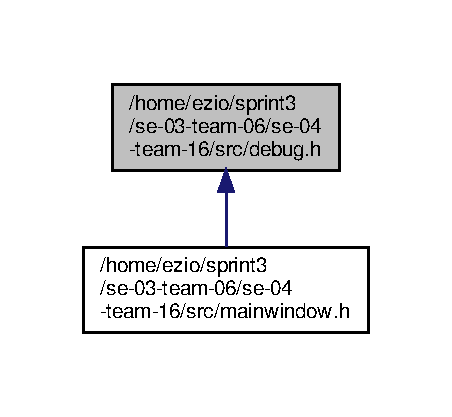
\includegraphics[width=217pt]{debug_8h__dep__incl}
\end{center}
\end{figure}
\subsection*{Classes}
\begin{DoxyCompactItemize}
\item 
class \hyperlink{classDebug}{Debug}
\begin{DoxyCompactList}\small\item\em Class to implement \hyperlink{classDebug}{Debug} functionality. \end{DoxyCompactList}\end{DoxyCompactItemize}


\subsection{Detailed Description}
This header file contains functionalities to debug the game. 


\hypertarget{intelligence_8h}{}\section{/home/fatine/\+Documents/se-\/03-\/team-\/06/src/intelligence.h File Reference}
\label{intelligence_8h}\index{/home/fatine/\+Documents/se-\/03-\/team-\/06/src/intelligence.\+h@{/home/fatine/\+Documents/se-\/03-\/team-\/06/src/intelligence.\+h}}


\hyperlink{classIntelligence}{Intelligence} currency implentation and functionalities.  


This graph shows which files directly or indirectly include this file\+:
% FIG 0
\subsection*{Classes}
\begin{DoxyCompactItemize}
\item 
class \hyperlink{classIntelligence}{Intelligence}
\begin{DoxyCompactList}\small\item\em Class to implement \hyperlink{classIntelligence}{Intelligence} currency. \end{DoxyCompactList}\end{DoxyCompactItemize}


\subsection{Detailed Description}
\hyperlink{classIntelligence}{Intelligence} currency implentation and functionalities. 


\hypertarget{mainwindow_8h}{}\section{/home/ezio/sprint3/se-\/03-\/team-\/06/se-\/04-\/team-\/16/src/mainwindow.h File Reference}
\label{mainwindow_8h}\index{/home/ezio/sprint3/se-\/03-\/team-\/06/se-\/04-\/team-\/16/src/mainwindow.\+h@{/home/ezio/sprint3/se-\/03-\/team-\/06/se-\/04-\/team-\/16/src/mainwindow.\+h}}


Main window functionality.  


{\ttfamily \#include $<$Q\+Main\+Window$>$}\newline
{\ttfamily \#include \char`\"{}pencil.\+h\char`\"{}}\newline
{\ttfamily \#include \char`\"{}production.\+h\char`\"{}}\newline
{\ttfamily \#include \char`\"{}wallet.\+h\char`\"{}}\newline
{\ttfamily \#include \char`\"{}intelligence.\+h\char`\"{}}\newline
{\ttfamily \#include \char`\"{}debug.\+h\char`\"{}}\newline
{\ttfamily \#include \char`\"{}server.\+h\char`\"{}}\newline
Include dependency graph for mainwindow.\+h\+:
\nopagebreak
\begin{figure}[H]
\begin{center}
\leavevmode
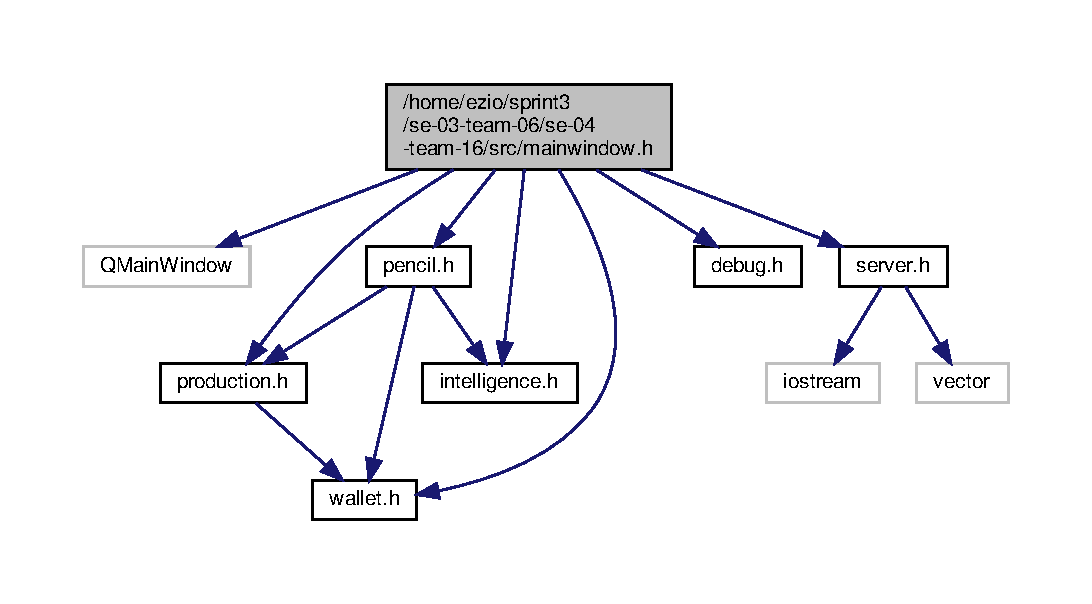
\includegraphics[width=350pt]{mainwindow_8h__incl}
\end{center}
\end{figure}
\subsection*{Classes}
\begin{DoxyCompactItemize}
\item 
class \hyperlink{classMainWindow}{Main\+Window}
\begin{DoxyCompactList}\small\item\em Class to implement the \hyperlink{classMainWindow}{Main\+Window}. \end{DoxyCompactList}\end{DoxyCompactItemize}
\subsection*{Namespaces}
\begin{DoxyCompactItemize}
\item 
 \hyperlink{namespaceUi}{Ui}
\begin{DoxyCompactList}\small\item\em Getting Main\+Wondow class from \hyperlink{namespaceUi}{Ui} namespace. \end{DoxyCompactList}\end{DoxyCompactItemize}


\subsection{Detailed Description}
Main window functionality. 


\hypertarget{pencil_8h}{}\section{/home/ezio/sprint3/se-\/03-\/team-\/06/se-\/04-\/team-\/16/src/pencil.h File Reference}
\label{pencil_8h}\index{/home/ezio/sprint3/se-\/03-\/team-\/06/se-\/04-\/team-\/16/src/pencil.\+h@{/home/ezio/sprint3/se-\/03-\/team-\/06/se-\/04-\/team-\/16/src/pencil.\+h}}


this header file contains the functionalities for buying and selling pencil and the Auto \hyperlink{classPencil}{Pencil} Machine (A\+PM).  


{\ttfamily \#include \char`\"{}production.\+h\char`\"{}}\newline
{\ttfamily \#include \char`\"{}wallet.\+h\char`\"{}}\newline
{\ttfamily \#include \char`\"{}intelligence.\+h\char`\"{}}\newline
Include dependency graph for pencil.\+h\+:
\nopagebreak
\begin{figure}[H]
\begin{center}
\leavevmode
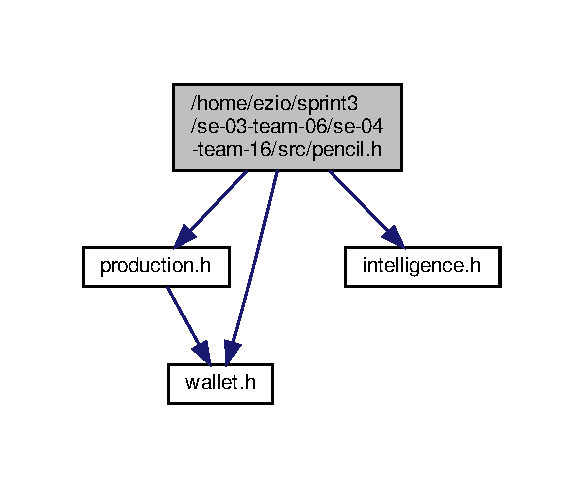
\includegraphics[width=280pt]{pencil_8h__incl}
\end{center}
\end{figure}
This graph shows which files directly or indirectly include this file\+:
\nopagebreak
\begin{figure}[H]
\begin{center}
\leavevmode
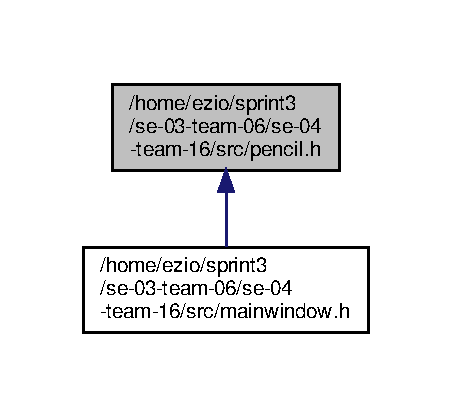
\includegraphics[width=217pt]{pencil_8h__dep__incl}
\end{center}
\end{figure}
\subsection*{Classes}
\begin{DoxyCompactItemize}
\item 
class \hyperlink{classPencil}{Pencil}
\begin{DoxyCompactList}\small\item\em Class to implement pencil game. \end{DoxyCompactList}\end{DoxyCompactItemize}


\subsection{Detailed Description}
this header file contains the functionalities for buying and selling pencil and the Auto \hyperlink{classPencil}{Pencil} Machine (A\+PM). 


\hypertarget{production_8h}{}\section{/home/fatine/\+Documents/se-\/03-\/team-\/06/src/production.h File Reference}
\label{production_8h}\index{/home/fatine/\+Documents/se-\/03-\/team-\/06/src/production.\+h@{/home/fatine/\+Documents/se-\/03-\/team-\/06/src/production.\+h}}


This header file contains functionalities to buy and sell wood and graphite.  


{\ttfamily \#include \char`\"{}wallet.\+h\char`\"{}}\newline
Include dependency graph for production.\+h\+:
% FIG 0
This graph shows which files directly or indirectly include this file\+:
% FIG 1
\subsection*{Classes}
\begin{DoxyCompactItemize}
\item 
class \hyperlink{classProduction}{Production}
\begin{DoxyCompactList}\small\item\em Class to implement production of the pencils. \end{DoxyCompactList}\end{DoxyCompactItemize}


\subsection{Detailed Description}
This header file contains functionalities to buy and sell wood and graphite. 


\hypertarget{wallet_8h}{}\section{/home/ezio/sprint3/se-\/03-\/team-\/06/se-\/04-\/team-\/16/src/wallet.h File Reference}
\label{wallet_8h}\index{/home/ezio/sprint3/se-\/03-\/team-\/06/se-\/04-\/team-\/16/src/wallet.\+h@{/home/ezio/sprint3/se-\/03-\/team-\/06/se-\/04-\/team-\/16/src/wallet.\+h}}


This header file contains required definitions for \hyperlink{classWallet}{Wallet}. It only stores Balance which is the money the user has in the bank.  


This graph shows which files directly or indirectly include this file\+:\nopagebreak
\begin{figure}[H]
\begin{center}
\leavevmode
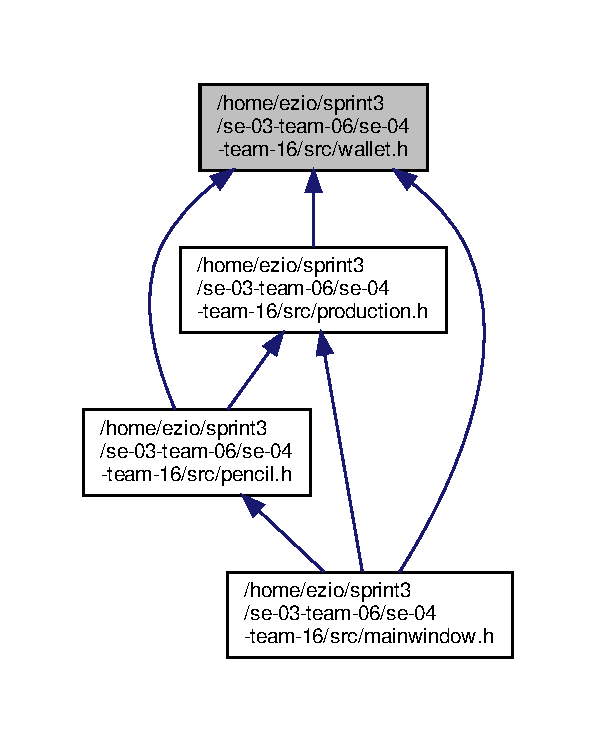
\includegraphics[width=286pt]{wallet_8h__dep__incl}
\end{center}
\end{figure}
\subsection*{Classes}
\begin{DoxyCompactItemize}
\item 
class \hyperlink{classWallet}{Wallet}
\begin{DoxyCompactList}\small\item\em Class to implement the wallet of the player. \end{DoxyCompactList}\end{DoxyCompactItemize}


\subsection{Detailed Description}
This header file contains required definitions for \hyperlink{classWallet}{Wallet}. It only stores Balance which is the money the user has in the bank. 


%--- End generated contents ---

% Index
\backmatter
\newpage
\phantomsection
\clearemptydoublepage
\addcontentsline{toc}{chapter}{Index}
\printindex

\end{document}
